\section{Conclusioni}

\begin{frame}
	\frametitle{Conclusioni}
	\begin{itemize}
		\setlength\itemsep{10pt}
		\item<1-> I 27 indici ETCCDI hanno permesso una migliore comprensione delle proiezioni climatiche future.
		\item<2-> Tutti gli indici di temperatura proiettano temperature più elevate.
		\item<3-> Gli indici di precipitazione proiettano aumento nella intensità.
		\item<4-> La variabilità dei modelli è maggiore sulle Ande.
    \end{itemize}    
\end{frame}	

\begin{frame}[t] \frametitle{Conclusioni}	
\begin{columns}
    \column[T]{0.5\textwidth} \vspace*{-3ex}
    \visible<1,3>{ 
        \begin{center}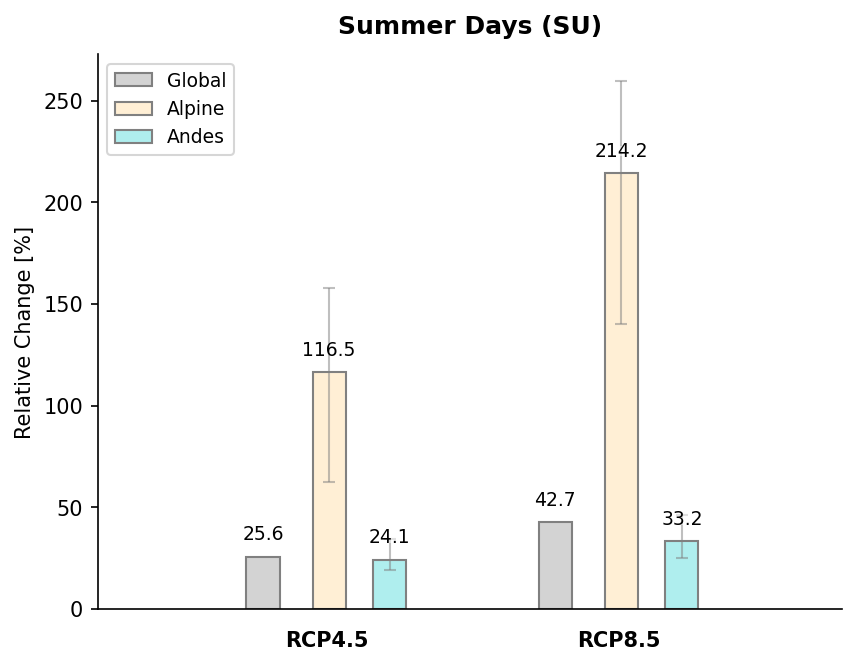
\includegraphics[width=\textwidth]{risultati/su_bar_rel}\end{center}
        \footnotesize Giorni d'estate ($T > 25$°C)            
    }    	
    
    \column[T]{0.5\textwidth} \vspace*{-3ex}
    	\visible<2,3>{
        \begin{center}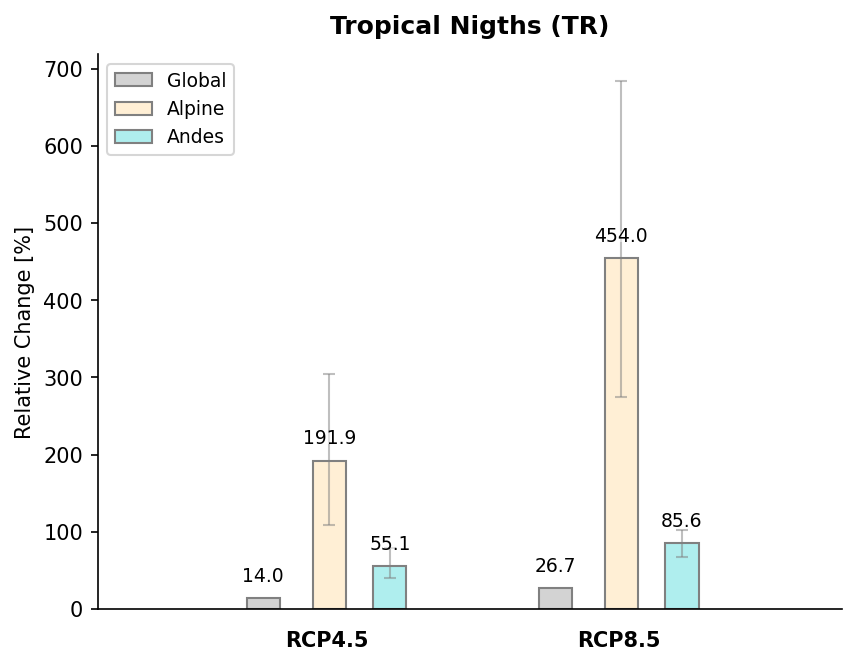
\includegraphics[width=\textwidth]{risultati/tr_bar_rel} \end{center}
    	    \footnotesize \hfill Notti tropicali ($T > 20$°C)         
    }
\end{columns}

        
\visible<3>{
    \begin{alertblock}{} Maggiore riscaldamento sulle Alpi.\end{alertblock}	
}
\end{frame}   
	
		
\begin{frame}[t] \frametitle{Conclusioni}	
\begin{columns}
    \column[T]{0.5\textwidth} \vspace*{-3ex}
    \visible<1,3>{ 
        \begin{center}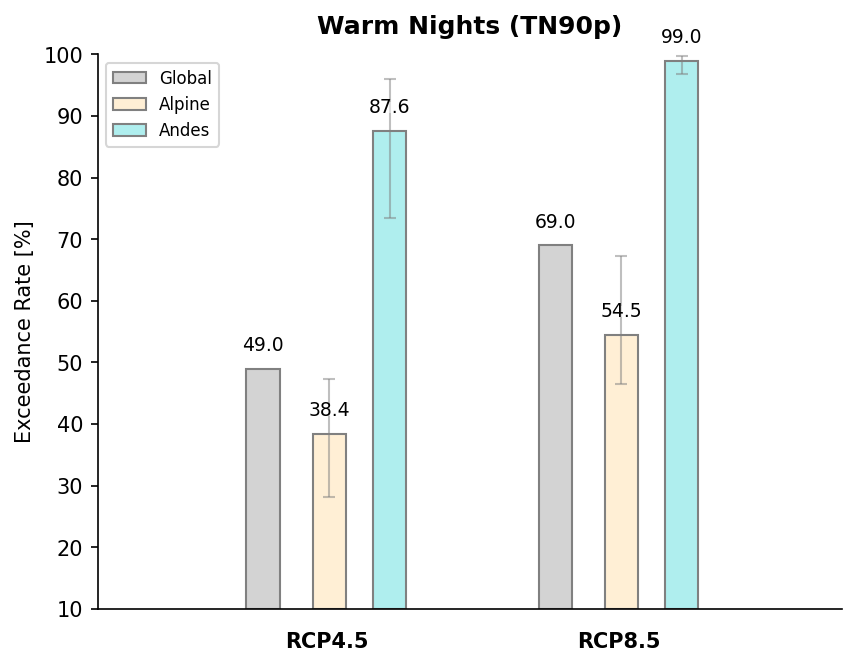
\includegraphics[width=\textwidth]{risultati/tn90p_bar_lim}\end{center}
        \footnotesize La percentuale di giornate/notte calde in un anno che nel periodo di riferimento era del 10\% (TX90p e TN90p)               
    }    	
    
    \column[T]{0.5\textwidth} \vspace*{-3ex}
    	\visible<2,3>{
        \begin{center}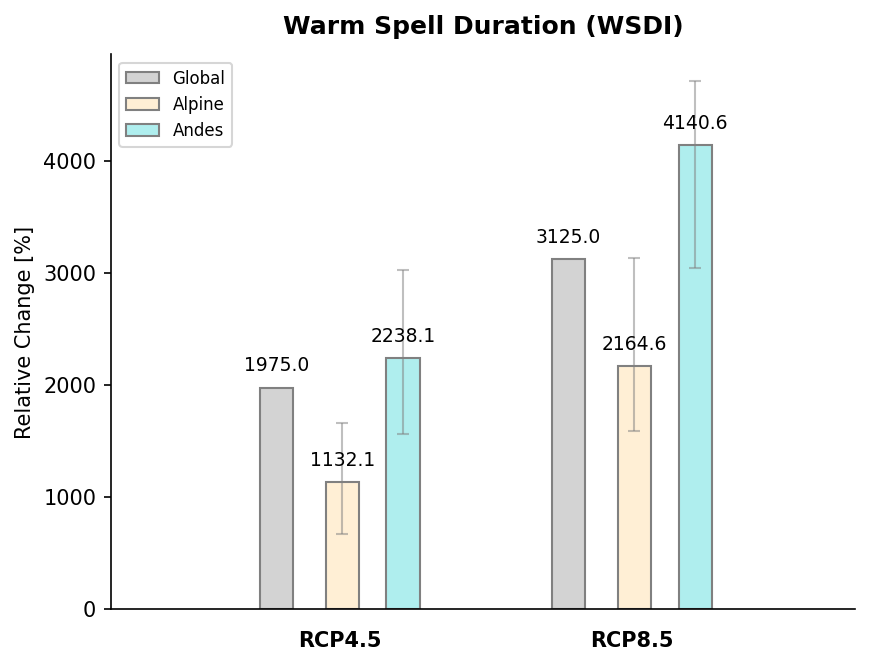
\includegraphics[width=\textwidth]{risultati/wsdieca_bar_rel} \end{center}
    	    \footnotesize \hfill La durata del periodo di calore (WSDI)          
    }
\end{columns}
        
\visible<3>{
    \begin{alertblock}{} Aumenterà in tutte le due regioni, maggiormente sulle Ande dovuto a la mancanza di stagioni.\end{alertblock}	
}
\end{frame}        



\begin{frame}[t] \frametitle{Conclusioni}	
\begin{columns}
    \column[T]{0.5\textwidth} \vspace*{-3ex}
    \visible<1,3>{ 
        \begin{center}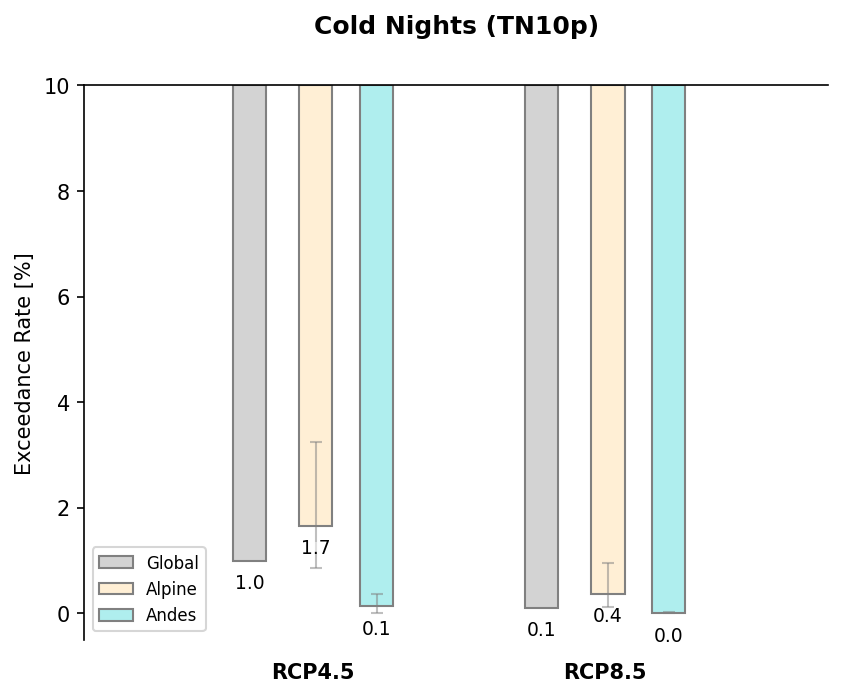
\includegraphics[width=\textwidth]{risultati/tn10p_bar}\end{center}
        \footnotesize La percentuale di giornate/notte fredde in un anno che nel periodo di riferimento era del 10\% (TN10p, TX10p)             
    }    	
    
    \column[T]{0.5\textwidth} \vspace*{-3ex}
    	\visible<2,3>{
        \begin{center}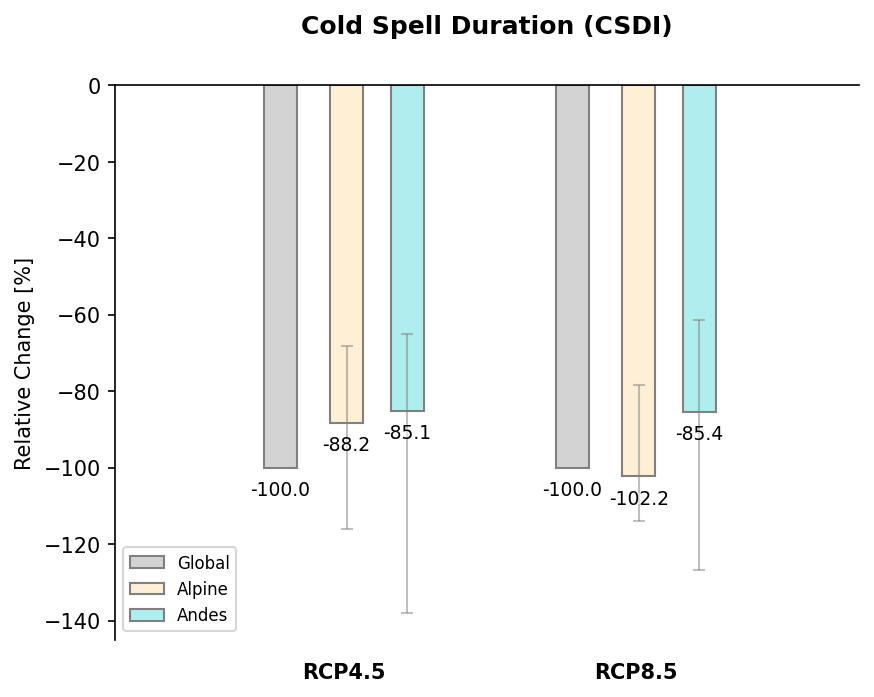
\includegraphics[width=\textwidth]{risultati/csdieca_bar_rel} \end{center}
    	    \footnotesize \hfill la durata del periodo freddo (CSDI)          
    }
\end{columns}
        
\visible<3>{
    \begin{alertblock}{} Indicano diminuzioni drammatici. Per lo scenario $8.5$, diminuzione totale sulle Alpi. \end{alertblock}	
}
\end{frame} 

		
\begin{frame}	
    \frametitle{Conclusioni}
    \begin{itemize}	
    \item<1-> La poca variabilità delle precipitazione totale annuale (PRCPTOT).
	\item<2-> La diminuzione del numero di giorni di pioggia (R1mm).  %indicano che in futuro aumenterà la frequenza (R20mm) e l'intensità (R99p) delle precipitazioni estreme (coerentemente alla relazione di Clausius-Clapeyron).
	\item<3-> La diminuzione di giorni di pioggia consecutivi (CWD).
	\item<4-> L'aumento dell'intensità delle precipitazioni (SDII). 
	\item<5-> L'aumento dei giorni di siccità consecutivi (CDD).
	\end{itemize}

\begin{alertblock}<6->{}
       \setlength\itemsep{0pt}
	  Aumenterà la frequenza e l'intensità delle precipitazioni estreme (coerentemente con l'aumento di temperatura come è spiegato dalla relazione di Clausius Clapeyron).
\end{alertblock}	
\end{frame}	
	
